\subsection{Introduction}


\subsection{Questions}
\subsubsection{Simulation}

\paragraph{Derive analytically the baseband model of the channel including the synchronisation errors.} The synch:
\begin{itemize}
\item a Carrier Frequency Offset (CFO) $\Delta \omega$
\item a phase offset $\phi_0$
\item a Sample Clock Offset (SCO) $\delta$
\item a time shift $t_0$
\end{itemize}
From these, one can update the baseband model as shown in figure~\ref{fig:sync}.

\begin{figure}[htbp]
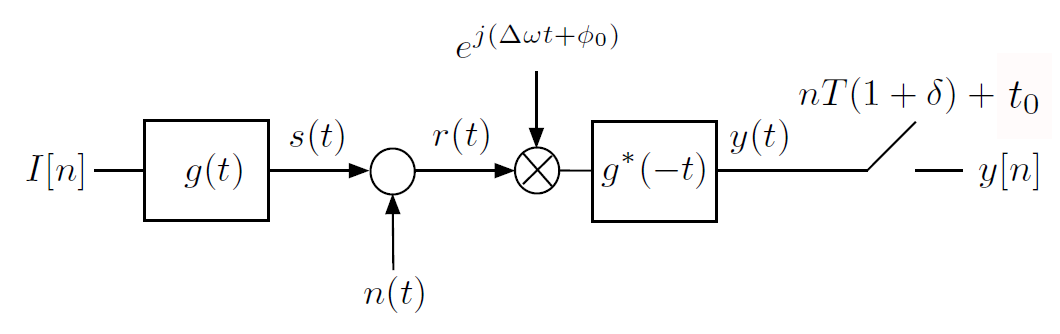
\includegraphics[width=\textwidth]{baseband_sync.png}
\caption{Baseband model with synchronization errors.\label{fig:sync}}
\end{figure}


\paragraph{How do you separate the impact of the carrier phase drift and ISI due to the CFO in your simulation?}
We do this by perfectly cancelling the CFO by hand after the filtering operation at the receiver.

\paragraph{How do you simulate the sampling time shift in practice?}The modulated message at the symbol frequency is first upsampled before all the other operations.
At the receiver, after the filtering operation, is signal is downsampled.
During this downsampling operation, a fixed sampling time shift can be introduced by shifting the indexes.

\paragraph{How do you select the simulated $E_{b}/N_{o}$ ratio?} Typical value of \SI{10}{\deci\bel} ? small enough to get something correct at the end and big enough to get some errors to be able to test our simulated channel with noise.

\paragraph{How do you select the lengths of the pilot and data sequences?} The pilot's length should be long enough to get a good estimation of the phase and the length of the data is selected to ensure a correct phase interpolation between two pilot sequences.

\subsubsection{Communication System}


\paragraph{In which order are the synchronisation effects estimated and compensated. Why?} First the sampling time shift is estimated and compensated with Gardner's algorithm, because frame and frequency acquisition can only work on a correctly sampled sequence, while Gardner's algorithm is robust to CFO.


\paragraph{Explain intuitively how the error is computed in the Gardner algorithm. Why is the
Gardner algorithm robust to CFO?} The algorithm works with a feedback structure. Each time shift estimate is the sum of the previous one and a weigthed version of the error. With a good selection of coefficient, the error on the phase converges to zero ...


\paragraph{Explain intuitively why the differential cross-correlator is better suited than the usual cross-correlator? Isn’t interesting to start the summation at $k = 0$ (no time shift)?}


\paragraph{Are the frame and frequency acquisition algorithms optimal? If yes, give the optimisation criterion.}
